\section{Original architecture}
The original architecture had a heavy emphasis on high throughput, as was the overall goal of the system.
Figure~\ref{fig:arch-orig} depicts the original design for system architecture.

\begin{figure}[tbph]
  \centering
  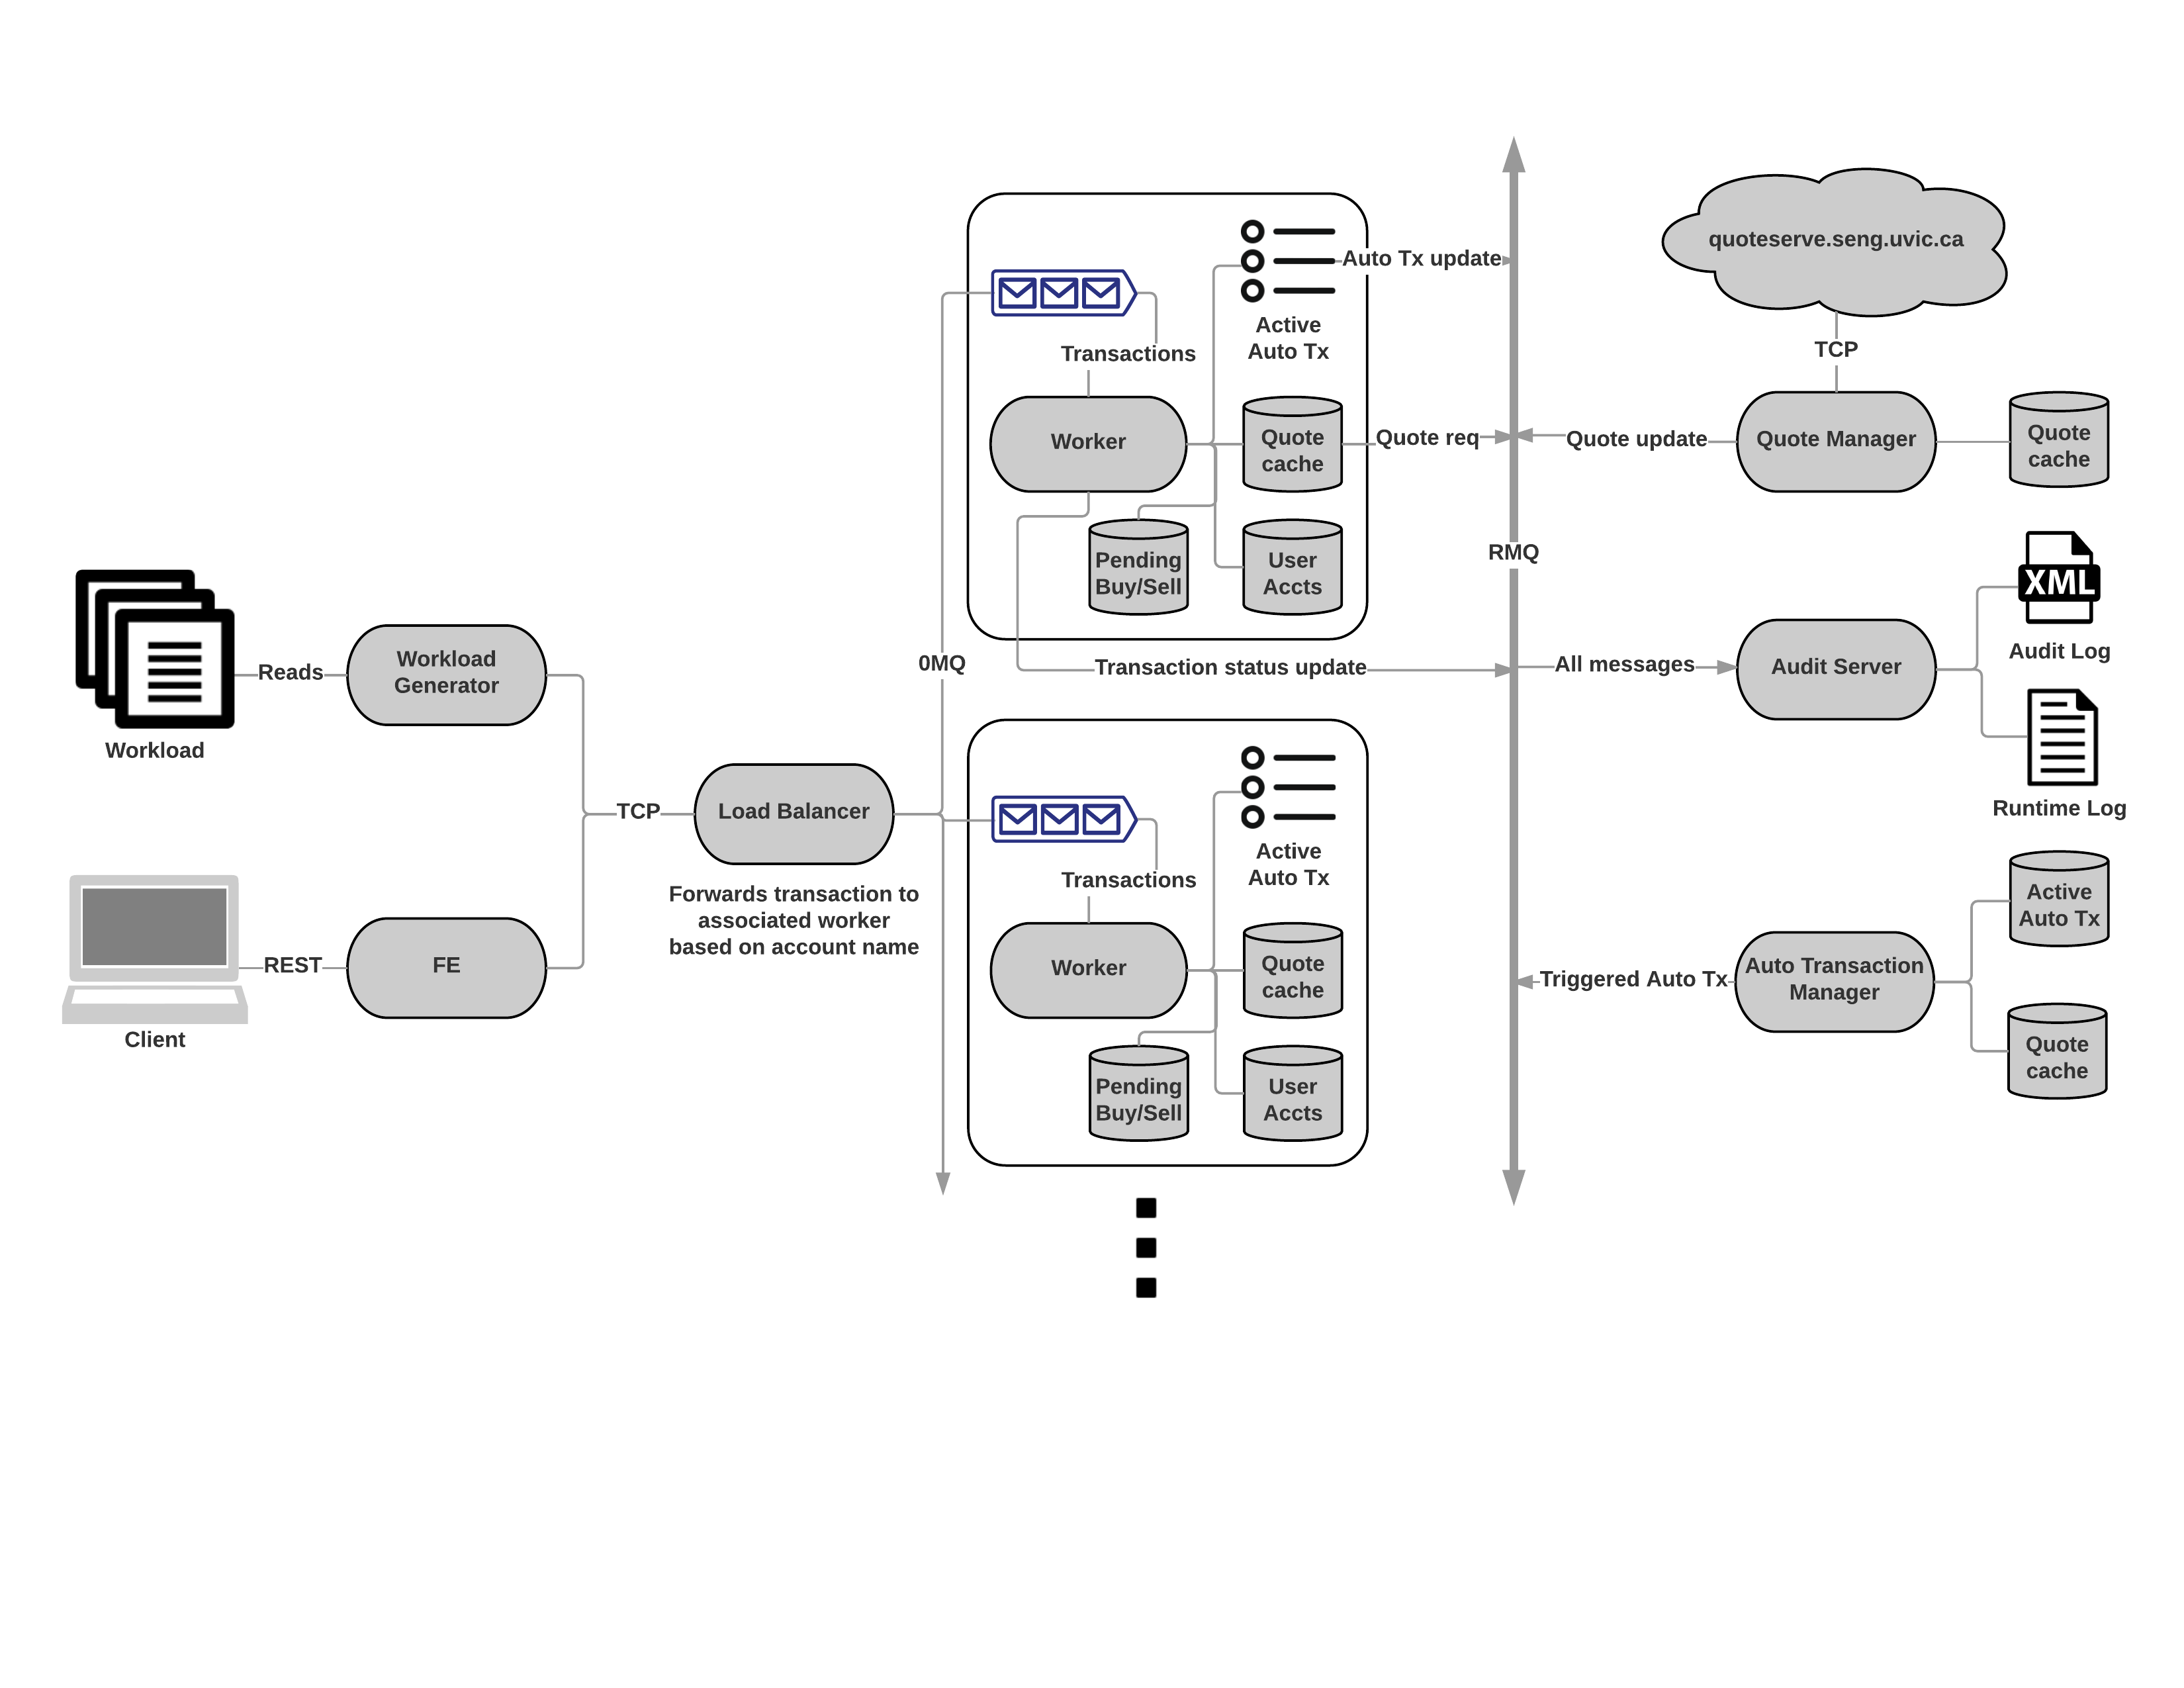
\includegraphics[width=0.85\linewidth]{../architecture/graphics/arch}
  \caption{Original system architecture}
  \label{fig:arch-orig}
\end{figure}


\paragraph{Incoming traffic}
Transactions will be sent to the load balancer at the TCP socket level, using a pre-defined serialization format very similar to what is provided in the workload files.

\paragraph{Client frontend}
A frontend server will host static-ish pages that allows clients to log in, view their accounts and execute trades.
Interaction should use REST but we'll probably end up sending data back and forth through web forms because it's faster to develop.
Amount of polish and technology choice will heavily depend on how quickly we can scale to a full workload.
Ideally, this should use a modern web development package like React or Vue.

Web page will do cursory input sanitization and validation (e.g.\ reject a purchase for negative dollars but checks against user account quantities such as stock holdings will occur later.)

\paragraph{Workload generator}
Reads a provided workload file and generates requests identical to those coming from the FE.
Requests will have a flag that indicates the transaction should run to completion but return no data.

\paragraph{Load balancer}
Forwards the transaction to its worker based on the user ID.
When the transaction is finished it returns the contents (which may only be an ACK) to the client.

The design goal for the load balancer is maximum throughput.
It should be a stateless router.
Zero Message Queue (0MQ) offers high throughput and a configurable broker that can scale horizontally.

\paragraph{Worker}
Transactions arrive from the load balancer and are place in a queue.
The worker parses the transaction and executes it.
It maintains user accounts (balance and stock holdings), a local quote cache and a list of active automatic transactions (ATXs).
All of the components of a worker live on the same machine.

Performance can be scaled horizontally by adding more workers.

\paragraph{Quote cache}
The quote cache maintains a list of all active quotes in the system by listening to broadcasts from the Quote Manager.
It will be implemented with a Redis store that uses TTL to automatically expire quotes.

\paragraph{User accounts}
There is no clear requirement for user accounts to exist on a persistent database.
The state of a user account is recoverable from the Audit Server.
There are no cross-account queries, aside from the system status dump that is performed by the Audit Server.
The first development cycle will use an in-memory data structure to hold user account data.
If performance suffers we'll examine a Postgres implementation.

\paragraph{Buy and sell}
Details for pending buy and sell actions will be stored in Redis with a TTL to enforce the transaction validity window.

\paragraph{Automatic transactions}
The worker maintains a list of each user's ATXs.
This list has no functionality other than mirroring the state of the consolidated Auto Transaction Manager (ATM) for the worker's accounts.
Updates to this list are echoed to the ATM for execution.
The worker is responsible for maintaining the validity of ATXs (e.g. an ATX is not valid if it receives a trigger without a pre-existing amount).

When an ATX triggers, the ATM notifies the worker that owns the ATX and the worker can update the account state and active auto transaction list.
This will be implemented on the same Redis store as the quote cache.

\paragraph{Logging}
Log events are sent to the Audit Server where they can be logged asynchronously.

\paragraph{Quote manager}
Serves concurrent requests for new quotes.
On its own cache miss (which should be rare because the cache state is maintained at the worker level through quote update broadcasts) it gets a new quote from the legacy service.
The fresh quote is stored into its local cache (Redis) and broadcast to all workers.

\paragraph{AutoTX manager}
Maintains a list of all active ATXs from workers.
It receives quote update broadcasts and checks if trigger conditions are satisfied.
Stocks that have not be refreshed recently will prompt to be updated.
Since multiple workers can have ATXs for the same stock the periodic price check can be amortized across all workers.

\paragraph{Audit server}
Records all bus traffic and unicast audit events from other services.

\paragraph{Audit log}
Logs external quoteserver hits and parsed transactions only.
The log will conform to the strict XML schema defined by Day Trading Inc.
The purpose of this log is for transaction per second evaluation only.

\paragraph{Runtime log}
Each event is logged to a single line using a custom logging format that associates log messages to exact lines of code.
This will provide a much finer grain event resolution than the audit log.

These events could be written to the audit log but the XML schema adds friction to log parsing.
For example, a single event is spread across an unknown number of lines making it very difficult to process logs line-by-line using standard Unix utilities like \texttt{grep}, \texttt{tail} and \texttt{awk}.
